\section{Data Integration and Assimilation Systems}
\label{se:dias}

\acrfull{dias} \cite{Kawasaki2018DataReduction} collects and archives data from satellites, weather stations, numerical forecasting models, and climate projection models. Once these data integrate into useful geographic information, DIAS generates results for managing global environmental problems and natural disasters \cite{Kawasaki2018DataReduction}. The DIAS can assimilate weather data from multiple data sources with different data formats. After successfully storing the data, it generates results which can be used for different kinds of purposes by other parties.

\begin{figure}[htp]
    \centering
    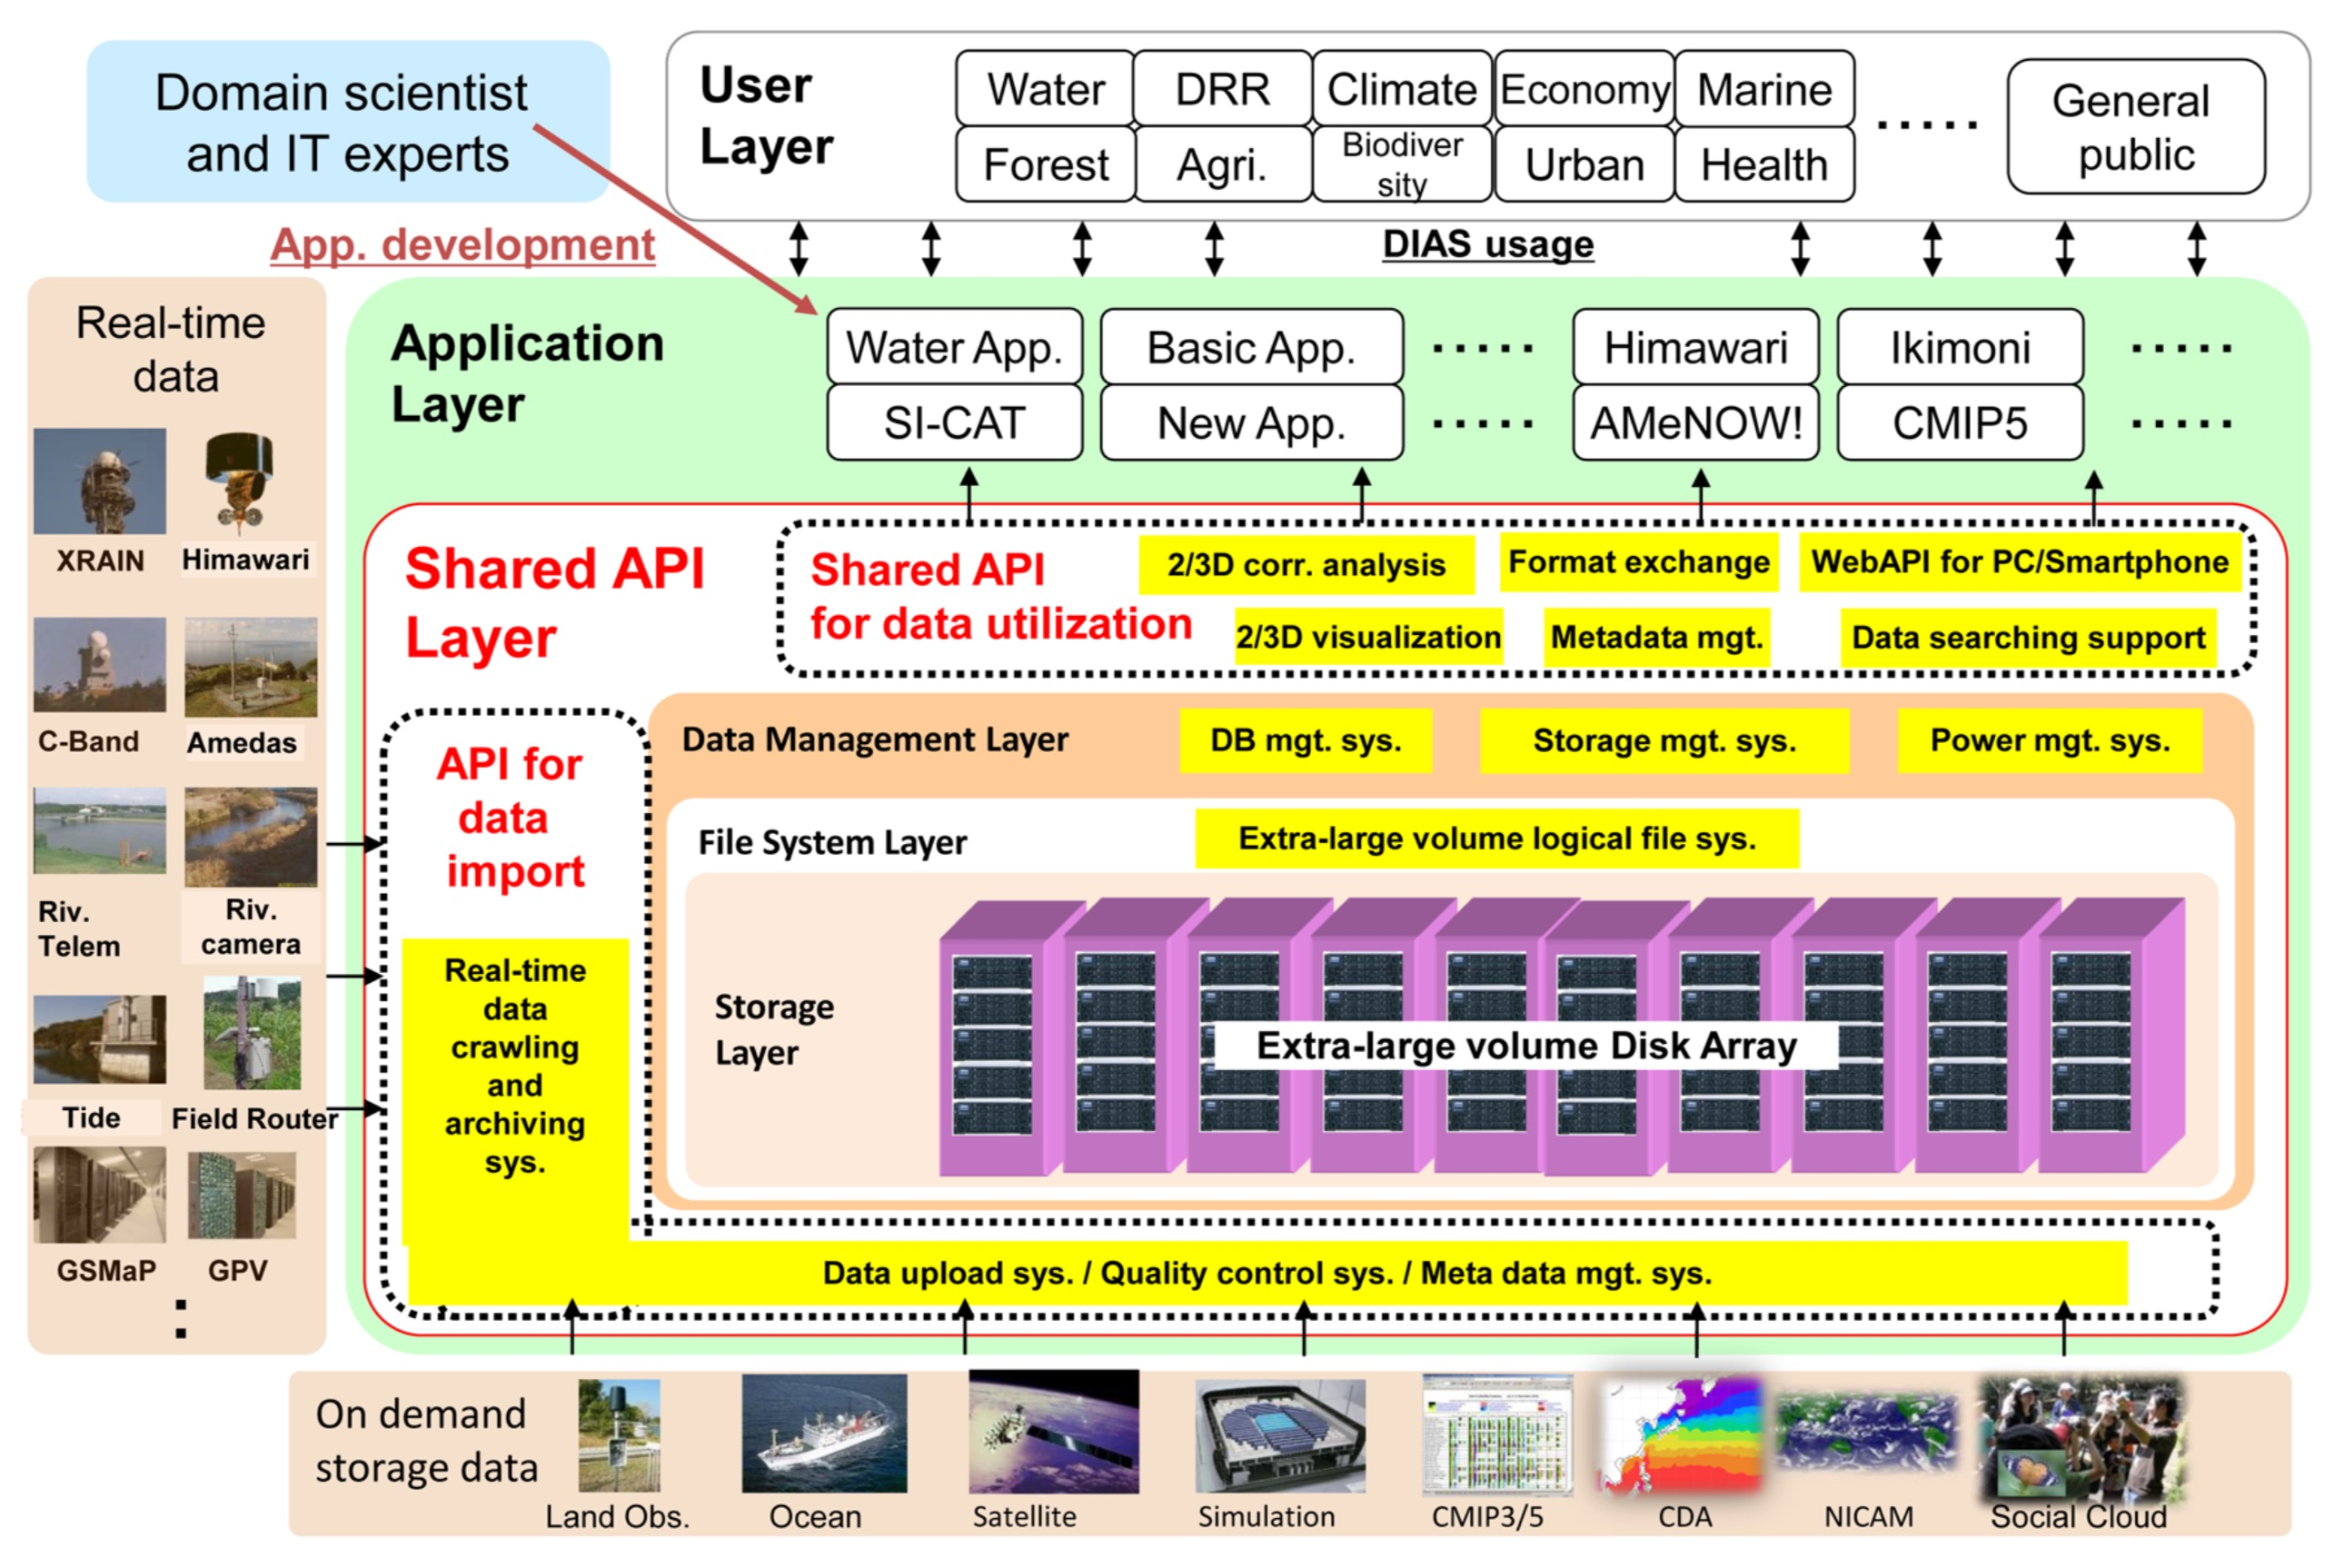
\includegraphics[width=1\textwidth]{lit/other/dias_common_base_application_platform.jpg}
    \caption[DIAS’s common base application platform.]{DIAS’s common base application platform \cite{Kawasaki2018DataReduction}.}
    \label{fi:dias_common_platform}
\end{figure}

The data storing mechanism is similar to the other systems discussed above. The DIAS provides an API to import the data and store them in a large array of storage after converting to the required data format. The APIs work to convert or reformat data into manageable forms and are useful for creating the DIAS storage archive. The DIAS's API contains various tools, including the real-time data exploration and archiving system, the data download system, the quality control system, and the metadata management system \cite{Kawasaki2018DataReduction}. To store on the large volume of disk space, it converts the data via a provided set of APIs. The above concept is similar to Delft-FEWs open data model approach. Further, the DIAS contains additional tools that provide the functionality of quality control of the data and metadata management, which is similar to some of the services in LEAD.

As shown in \cref{fi:dias_common_platform}, it offers an application layer that allows scientists to work on research tasks and to develop specific tools and applications by collaborating with IT experts \cite{Kawasaki2018DataReduction}. Once the data is stored on the DIAS system, it shares those data via the Shared API layer and allows users to remote access to the data and easy integration via the APIs.


%%%%%%%%%%%%%%%%%%%%%%%%%%%%%%%%%%%%%%%%%%%%%%%%%%%%%%%%%%%%%%%%%%%%%%%%%%%%%%%%
\section{Meteorological Assimilation Data Ingest System}
\label{se:madis}

\acrfull{madis} \cite{Macdermaid2005ArchitectureP2.39} is a data integration and assimilation system that collects data from dozens of suppliers, then checks the quality of the data and saves it in \acrshort{netCDF} format. Later, users can access the data with the support of the different types of data access protocols.

\begin{figure}[htp]
    \centering
    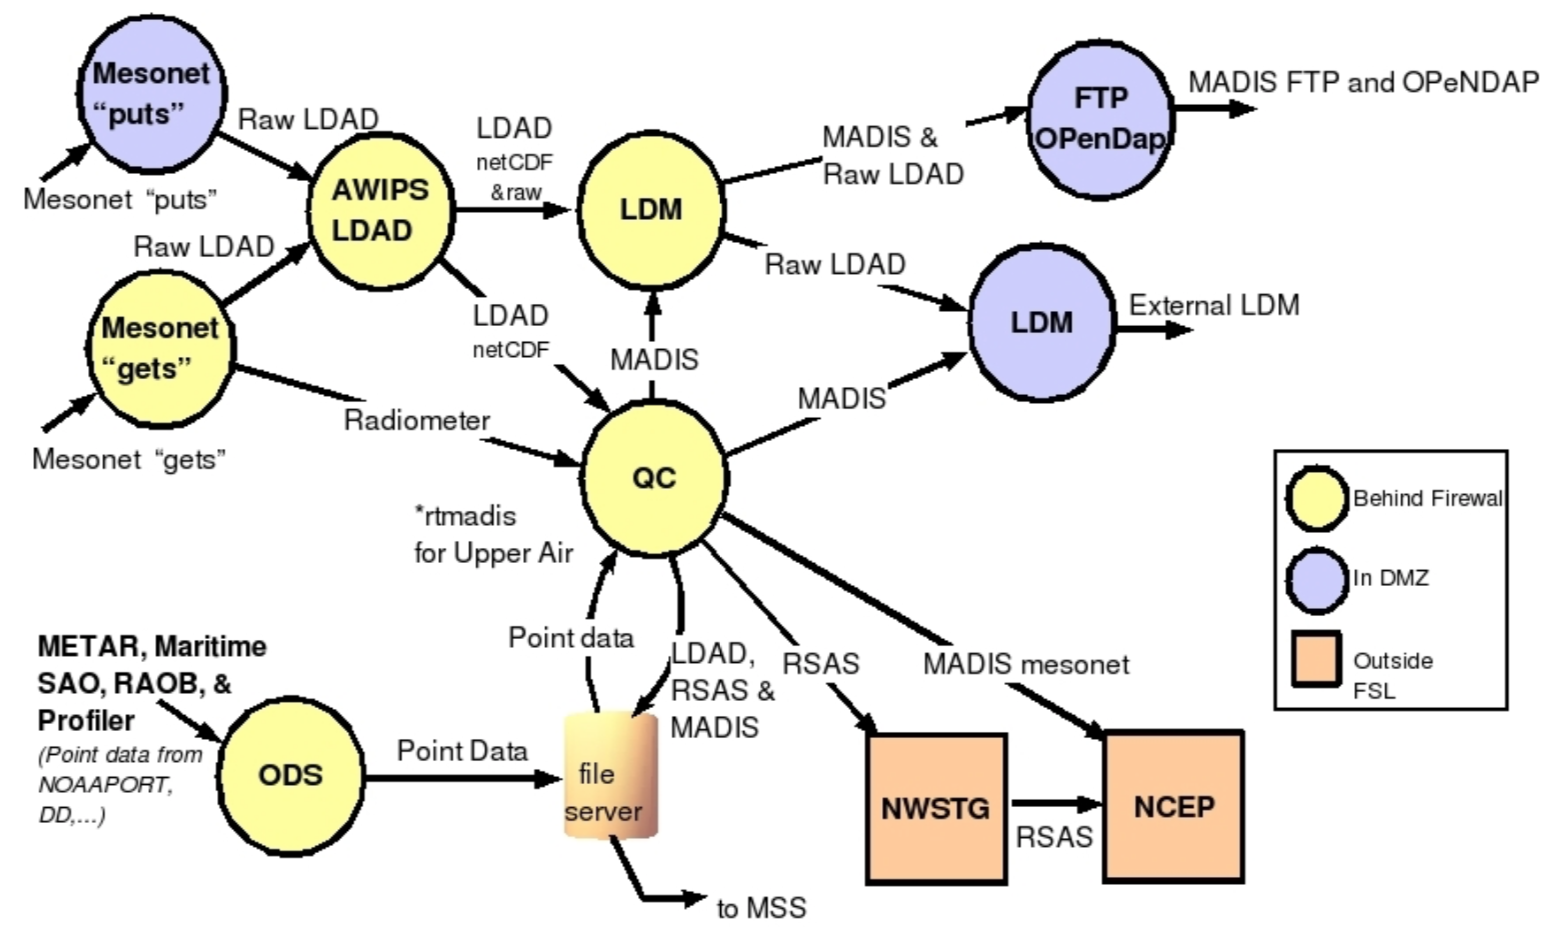
\includegraphics[width=1\textwidth]{lit/other/madis_flow.png}
    \caption[\acrshort{madis} data flow]{\acrshort{madis} data flow \cite{Macdermaid2005ArchitectureP2.39}.}
    \label{fi:madis_flow}
\end{figure}

MADIS contains a distributed architecture for data acquisition, processing, and distribution functions. Besides, the MADIS was developed based on the distributed architectural patterns available at the time of implementation. The various functional hosts have been paired using Linux High Availability (HA) to provide automated failover in the event of a system failure. It uses several methods for data dissemination such as FTP, Local Data Manager (LDM), and the Web OPeNDAP (OPen source project for Network Data Access Protocol) \cite{Macdermaid2005ArchitectureP2.39}. It uses functional calls like Remote Procedure Call (RPC) to invoke among the cluster of nodes. In \cref{fi:madis_flow}, the data is transported from the input and preprocessing systems to the central computer systems and then to other hosts for storage and distribution \cite{Macdermaid2005ArchitectureP2.39}. To get high availability, it has added some updates to its architecture, as mentioned in the paper.

Based on the above statements, we can conclude that these kinds of functionalities are available at the modern Cloud Computing tools, and out of the box, those tools are providing the scalability and high availability. Using those tools, it is possible to implement such a system with less effort and high confidence.

The MADIS regularly acquires Mesonet data from dozens of network providers representing more than 14,000 stations, and the system translates into more than 30,000 station reports every hour. Different systems that work inside and outside the firewall collect the data. The collected data is sent to the data server of the Advanced Weather-Interactive Processing System (AWIPS) of the central installation for processing and conversion to a common data format, NetCDF. The NetCDF files are then transferred to MADIS compute nodes \cite{Macdermaid2005ArchitectureP2.39}. After reading the statistics of the MADIS system, I realized the paper is a useful reference for system architecture design and its performance testing. When compared to the Delft-FEWS, the MADIS also converts the assimilated data into netCDF format. After converting to netCDF format, the netCDF files are transferred to the compute nodes and accessible via OPeNDAP. Many of these computers are configured using Linux clustering with high availability \cite{Macdermaid2005ArchitectureP2.39}.

Some of the MADIS data is considered to be the property of the supplier, and data access should be provided based on the authorization. In order to address the issue, MADIS data is divided into six different versions, depending on the access level authorized by the data provider \cite{Macdermaid2005ArchitectureP2.39}. When compared to Delft-FEWS, MADIS provides control-based access to the data.

%%%%%%%%%%%%%%%%%%%%%%%%%%%%%%%%%%%%%%%%%%%%%%%%%%%%%%%%%%%%%%%%%%%%%%%%%%%%%%%%
\section{Summary}
\label{se:lit_summary}

We presented several related works on WDIA system implementations such as \acrshort{fews}, \acrshort{lead}, \acrshort{dias}, and \acrshort{madis}. During our research, one of the significant issues that we focused on, store the data ingested from different sources with different formats efficiently. The Delft-FEWS and MADIS are using the netCDF as the common data format to store the data, which is one of the best solutions available with modern technologies as well. Even the LEAD and DIAS papers are not mentioned directly; those systems are also following a method of having common storage space to store bulk data. The Delft-FEWS and LEAD have the capability of handling the workflow of forecasting, but other systems are mainly focused on providing a weather data management system. The Delft-FEWS provides a modular approach via its general adapter, and according to the \acrshort{soa} architecture of LEAD provides the same functionality via services.

Above WDIA systems are developed with the contributions from lots of researchers, and were implemented specifically to address issues like natural disasters. A use case such as CUrW, a given WDIA system requires to remodel the systems and define the forecasting flows to support the country-specific requirements. Even some of the systems try to follow a generic approach to integrate new modules, but it is challenging to deploy modules for a closed source or proprietary software. Further, most of the systems depend on the underline software platform and do not support more resource-efficient and highly-scalable technologies such as cloud computing.
